\documentclass[a4j]{jsarticle} %jsrticleでもいい
\usepackage{fancyhdr} %ヘッダーを表示させるのに必要
\usepackage{listingsutf8}%日本語
\usepackage{color}
\usepackage{comment} %複数行のコメントアウトのパッケージ
\usepackage{amsmath,amssymb}
\usepackage[dvipdfmx]{graphicx}
\usepackage{here}
\usepackage{ascmac}
\usepackage{subfigure}%画像を横に配置
\setlength{\parindent}{0pt}


\pagestyle{fancy}
  \lhead{メディア情報学プログラミング演習} %ヘッダー左
  \rhead{J1-26} %ヘッダー右
\topmargin =-15mm %ページ上部の隙間の調整

\title{令和6年度 メディア情報学プログラミング演習\\グループプログラミング レポート\\料理提供ゲーム「MiniCook」}
\renewcommand{\lstlistingname}{コード}
\begin{document}
\maketitle

\begin{center}%中央に表書く
  \begin{tabular}{|c||c|}
      \hline
      学科&情報理工学域\\
      \hline
      クラス&J1\\
      \hline
      グループ番号&26\\
      \hline
      2210259&米谷祐希\\
      \hline
      2210730&鈴木早紀\\
      \hline
      2210743&吉田陽音\\
      \hline
  \end{tabular}
\end{center}

\newpage

\section{概要説明}
 このゲームは、レストランで働くプレイヤーが、制限時間内に料理を作るゲームである。以下の料理提供までの手順を繰り返すことでポイントを獲得し、制限時間終了時にスコアとランクが表示される。
\begin{enumerate}
  \item オーダーの確認\par
   まず、画面上部にランダムにオーダーが提示される。オーダーには、使う食材と調理方法が記載されている。各オーダーにはそれぞれ制限時間が設定されており、残り時間はオーダー上のゲージにリアルタイムに表示される。
  \item 食材の調理\par
   次に、オーダーに記載されている食材を、各食材ボックスから取り出す。各食材を持ったまま、各調理器具の前でアクションボタンを押すことで、食材が加工される。
  \item 料理の完成と提供\par
   料理は、加工された食材とお皿を組み合わせることで完成する。それらを組み合わせて料理ができあがれば、提供口に置くことで提供となり、オーダーと一致しているか判定される。一致していれば加点、間違っていれば減点となる。   
\end{enumerate}
 また、ゲームは3画面に分かれており、スタート画面、ゲーム画面、リザルト画面がある。また、各画面や各動作にはBGMや効果音がついている。操作はキーボードのA,S,D,W,J,K,Spaceキーを用いている。\par
 作業はGitHubを用い保存・共有を行った。米谷がModelと全体の管理、鈴木がView、吉田がControllerを主に担当したが、最終的には各自の担当領域を超えて協力しながら取り組んだ。
文責:鈴木

\section{設計方針}
 図1にクラス図を示す。%%%%%%%%%%%%%%%%%%%%%%%%%%%%%
\begin{figure}[H]
  \begin{center}
  
\includegraphics[width = 135mm]{img/class_graph.png}
  \caption{クラス図}
  \end{center}
\end{figure}
 クラス図に示しているように、MiniCookというクラスが大元のクラスとなっている。
その中でインスタンスとして5つのクラスを保持している。
Startクラス・Resultクラスはゲーム開始前の画面と、ゲーム終了時にスコアの表示等を行うためのクラスである。
そして設計方針について、このゲームはプレイヤーがオーダーに従って各種料理をつくる。
その中で、プレイヤーは皿や食材をいろんな座標に置くというプロセスが起きる。それに適応、そして拡張性を保つような構成にした。詳細に関しては以下で説明する。
今回のプログラムは大量生産するインスタンスが存在しないという想定を最初の構想で予測したためObserverモデルは用いずに、基本的なMVCモデルを元にして作成した。
\begin{itemize}
  \item Model\par
   DrawModelクラスでは、各種データの管理とそれに伴ったメソッドの提供をおこなった。基本的にゲームの情報は各種クラスからModelに参照されて提供する。
  Player,Gridなどの基盤にあるようなクラスはここでインスタンスを作成している。
  \item View\par
   DrawViewでは、Modelクラスより取得した情報を元に一括で描画処理を行う。
  フィールドのどの場所にどの物を描画するかの元情報をModelより取得。
  その後その情報を元に画像をViewクラスのメソッドを用いて判定して、画像を選択・描画している。
  当初の予定では、完全に2Dでゲームを作成する予定であったが、途中で擬似3Dにして立体感を出そうという構想が生まれた。
  しかしViewモデルで一括で管理しているおかげで、プログラムの書き直しは最低限に抑えることができた。
  \item Controller\par
   DrawControllerクラスでは、基本的にはプレイヤーからの入力の受取のみを行う。
  それぞれキーボードの入力を受取、それに応じた動作をそれぞれのクラス内のメソッドでおこなってもらう。\\
   しかしゲームに動的なアニメーションを少し付ける都合でキー入力を行いたいときと行いたくないときがある。
  それに対応するために、あるクラスのメソッドを呼び出すときもあれば、キー入力中にbooleanのフラグを用いて、動作先で参照してもらう形になっているものもある。
  \item Player・Grid\par
   この2つのクラスは、このプログラムのいちばん重要なクラスである。
  名称が違うもののプレイヤーが食材を保持している場合とあるマス目が食材を持っている(食材を置いている)という違いがあるのみで、ほとんど同じものである。
  このクラスでは、そのマスないしはプレイヤーがなにを持っているかというクラスをインスタンス変数に保持している。そして、Playerに許された行動やGrid(マス目)によってできる。
  行動についての自身の情報を持っており、それに対応したメソッドを提供している。
  \item Order\par
   Orderクラスでは、画面上部に定期的なタイミングで出現する、提供しなければならない料理の情報を持っているクラスである。
  注文1つごとにこのクラスが生成されて、その中にオーダーの制限時間、必要な材料などの情報をしている。
  \item Food\par
   このFoodクラスが、食材に関しての最小単位となるクラスである。抽象クラスという定義をしており、これを継承してキャベツであったり、トマトであったりのクラスを作成している。
  それぞれ継承されたクラスにおいて。それぞれ特有の調理される方法や、調理された情報を保持することができる。これを複数個ミックスして料理となったものが後述するPlateクラスである。
  \item Plate\par
   このPlateクラスでは、Foodクラスをいくつか保持していて、それによって例えばキャベツとトマトのサラダであったり、魚の切り身と海苔で巻き寿司といったものになる。
  これがOrderに存在していれば正解、なければ不正解という形である。
  また各マス目とPlayerはFoodクラスを単体で保持して食材を持っていたり、Plateクラスを持っていて、複数の食材からなる料理を持っていたりする。
  なお正誤判定についてはOrderクラスで行わずこちらでOrderクラスの内容をModelを経由して取得して、自分との合致があるかどうかで行っている。
\end{itemize}
 クラス間の関係と全体の参照の流れを説明する。ほどんどの基本の流れはModelクラスを参照して行われる。
ユーザーからの入力はDrawControllerからModelへ、描画はModelを参照してDrawVierクラスな内で行われる。
プレイヤーは移動をして該当の場所に移動してアクションを行うことで、Foodクラスを新たに生成したり、その場においたり、またそれらを調理してまとめてPlateクラスに保持する。
それを提出口に提出した際に、現存しているオーダーとの正誤判定を行いスコアのアップダウンを行う。ここでは説明を省略したが、各種タイミングでSEやBGMを鳴らすようなコードも含まれている。
\\文責:米谷




\section{プログラムの説明}
 以下にクラスとその説明を示す。
\begin{itemize}
  \item MiniCook\par
   %%%%%%%%%%%%%%%%%%%%%%%%%%%%
  \item Model\par
   %%%%%%%%%%%%%%%%%%%%%%%%%%%
  \begin{itemize}
    \item Food\par
     このFoodクラスは、料理の食材を表現するための抽象クラスである。インスタンス変数として、食材の状態を整数値で表現するためのfoodStatu、それぞれの調理法が可能かどうかを示すフラグであるcanCut、canHeat、食材が皿の上にあるかどうかを示すフラグisPlate、食材の名前を保持するための文字列foodNameを持つ。コンストラクタでは継承した子クラスの食材に併せて初期化が行えるように実装している。

    文責:吉田
    \item Order\par
     このOrderは、料理の注文を管理するクラスである。注文の基本情報を保持するインスタンス変数として、注文の名前を文字列で管理するorderName、何個目のオーダーであるかを表すorderIndex、アニメーション用の座標を表すposAnim、subOrderPosY、subOrderPosYAnimを持つ。また、食材に関するインスタンス変数として、皿を持っているかのフラグであるhasPlate、必要な食材を表すingeredient1~3がある。さらに、注文の制限時間であるtimeLimit、注文が生成された時間を示すcreateTime、自動削除用のタイマーであるexpirationTimerをインスタンス変数として持つ。制限時間が経過した場合は、効果音を鳴らし、スコアを下げ、注文が削除される。

     コンストラクタでは注文の名前や必要な食材、制限時間を注文ごとに設定できるようになっている。

     注文の完成判定を行うisCompletedメソッドはPlateクラスのオブジェクトを引数に持つ。プレイヤーが作った料理であるplate.foodと注文の材料であるorderIngredientsを1つずつ比較して、一致していれば判定用の配列をtrueとする。全ての食材が揃っていればtrueを返す。

     残り時間を計算するメソッドとしてgetRemainingTimeがある。これは現在時刻から注文作成時刻を引くことで経過時間を計算し、timeLimitから経過時間を引くことで残り時間を取得する。

     getRemainingTimeが0以下であるかで注文の期限切れを判定するisExpiredメソッドと、手動で注文を削除する際にタイマーを停止するためのcancelTimerメソッドも用意している。

    文責:吉田
  \end{itemize}   
  \item View\par
   %%%%%%%%%%%%%%%%%%%%%%%%  
  \begin{itemize}
    \item Timer\par
     %%%%%%%%%%%%%%% 
    \item Image\par
     %%%%%%%%%%%%%%%%%%%%%%%%%
    \item Player\par
     %%%%%%%%%%%%%%%%%%%%%%%%%
    \begin{itemize}
      \item Plate\par
       %%%%%%%%%%%%%%%%%%%%%%%%% 
      \item Grid\par
       %%%%%%%%%%%%%%%%%%%%% 
    \end{itemize}   
  \end{itemize}  
  \item Controller\par
   %%%%%%%%%%%%%%%%%%%%%%%%%%% 
  \item Start\par
   %%%%%%%%%%%%%%%%%%%%% 
  \item Result\par
   %%%%%%%%%%%%%%%%%%%%%%%%% 
  \item CardLayout\par
   %%%%%%%%%%%%%%%%%%%%%%%%%%% 
  \item AudioManager\par
   %%%%%%%%%%%%%%%%%%%%%%%%%%%% 
\end{itemize}
文責:%%%%%%%%%%%%%%%%%%%%%%%%%%%%%%



\section{実行例}
\subsection*{スタート画面}
 実行すると始めにこの画面(a)が現れる。スタートボタンを押すとゲーム画面:スタート時(c)になる。
\subsection*{リザルト画面}
 ゲーム終了後はこのリザルト画面(b)になる。スコアによってランクが星の数で表される。
\subsection*{ゲーム画面:スタート時}
 スタート時の画面(c)では、食材などは何もなく、オーダーが1つ入るところから開始される。上部にはオーダー、中央にはゲーム部分、下部にはスコアと制限時間を表示している。
\subsection*{ゲーム画面:オーダー}
 画面上部のオーダー(d)では、完成品、必要な食材、加工方法、残り時間が示されている。
\subsection*{ゲーム画面:加工前}
 加工前の食材(e)をボックスから取り出す。
\subsection*{ゲーム画面:加工後}
 調理器具でアクションを行うと加工後の画像(f)に切り替わる。
\subsection*{ゲーム画面:組み合わせ}
 皿の上に各食材を載せると画像がそれに伴い完成品(g)となる。
\subsection*{ゲーム画面:提供}
 完成した料理を提供口に置くと、ホールスタッフが取りに来る(h)。
\newpage
\begin{figure}[H]
  \begin{center}
    \subfigure[スタート画面]{
      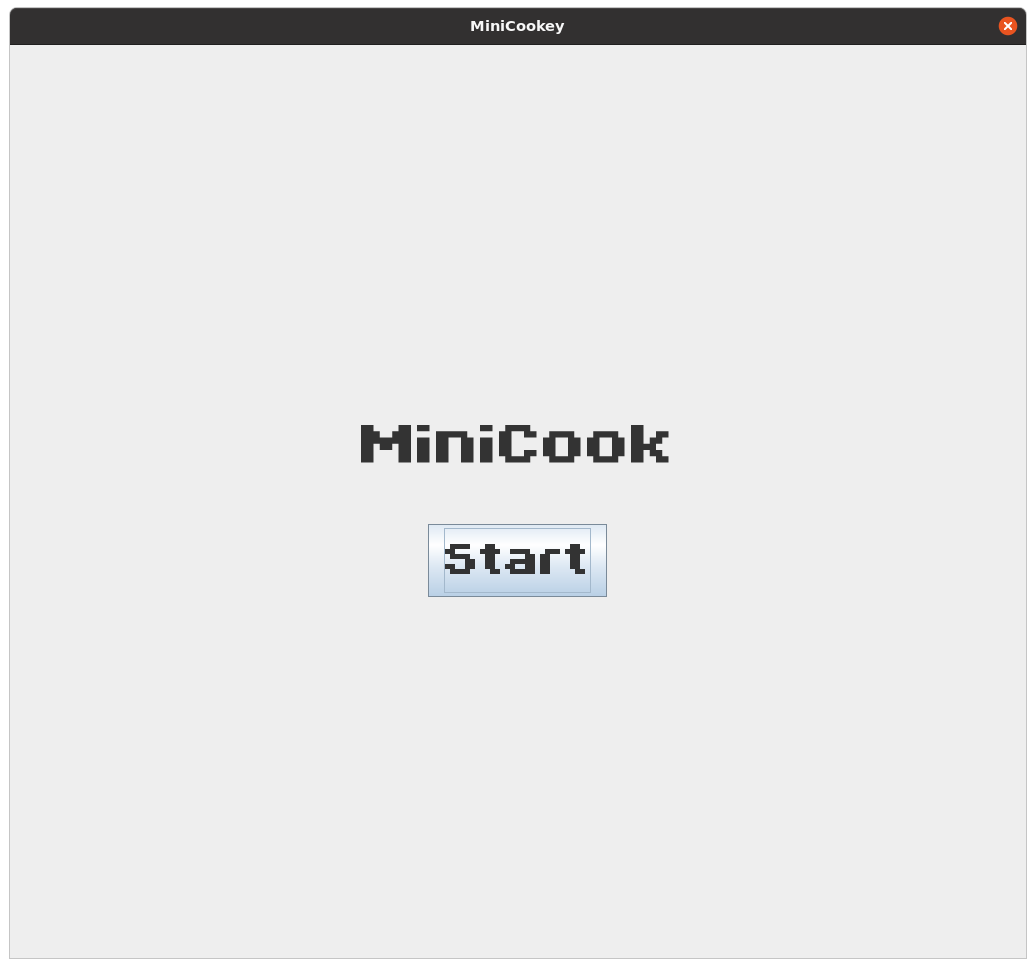
\includegraphics[width=0.4\textwidth,keepaspectratio]{img/a.png}
    }
    \subfigure[リザルト画面]{
      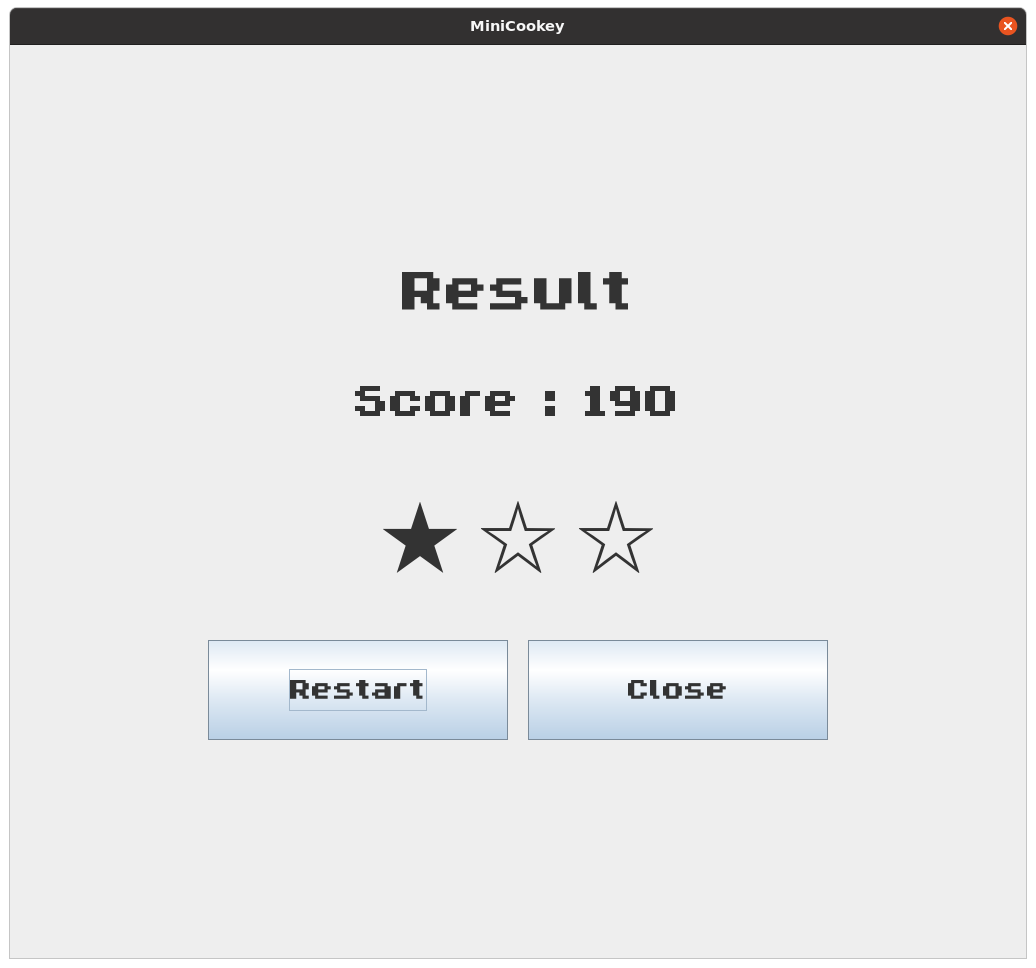
\includegraphics[width=0.4\textwidth,keepaspectratio]{img/b.png}
    }
  \end{center}
\end{figure}
\begin{figure}[H]
  \begin{center}
    \subfigure[ゲーム画面:スタート時]{
      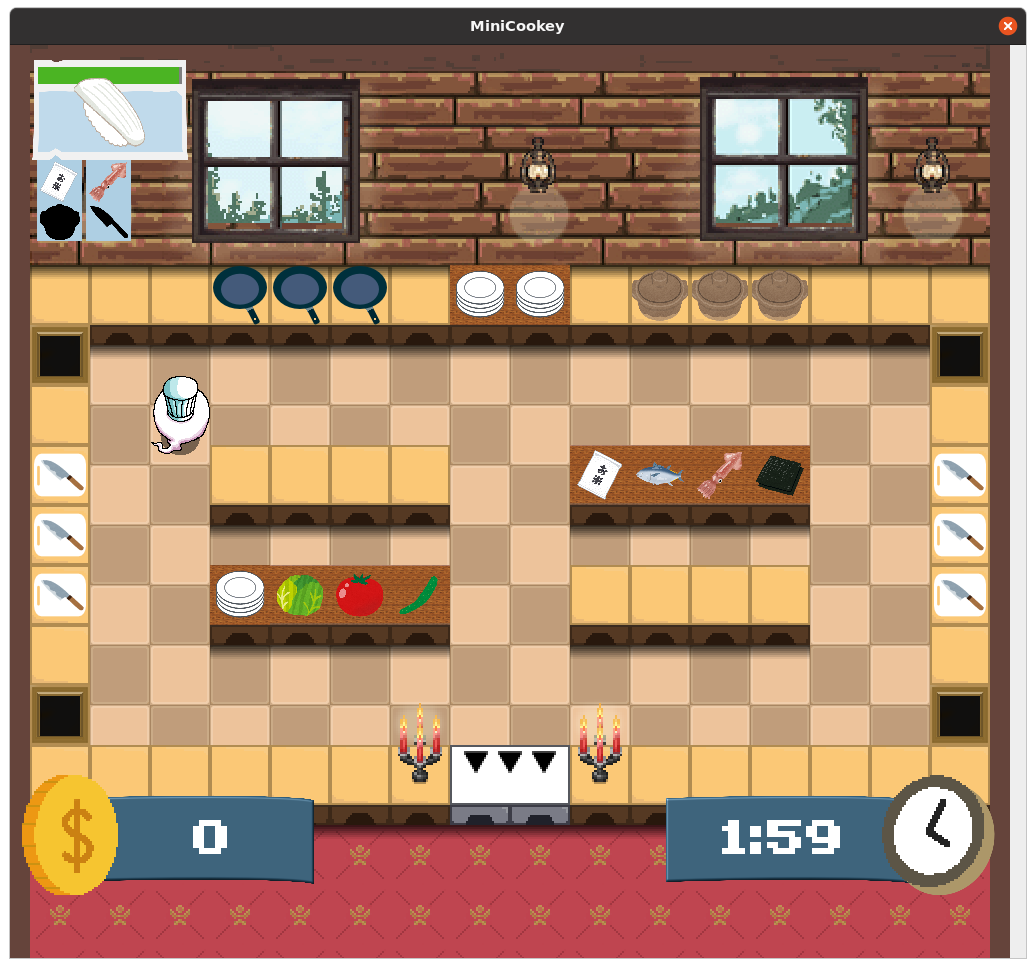
\includegraphics[width=0.4\textwidth,keepaspectratio]{img/c.png}
    }
    \subfigure[ゲーム画面:オーダー]{
      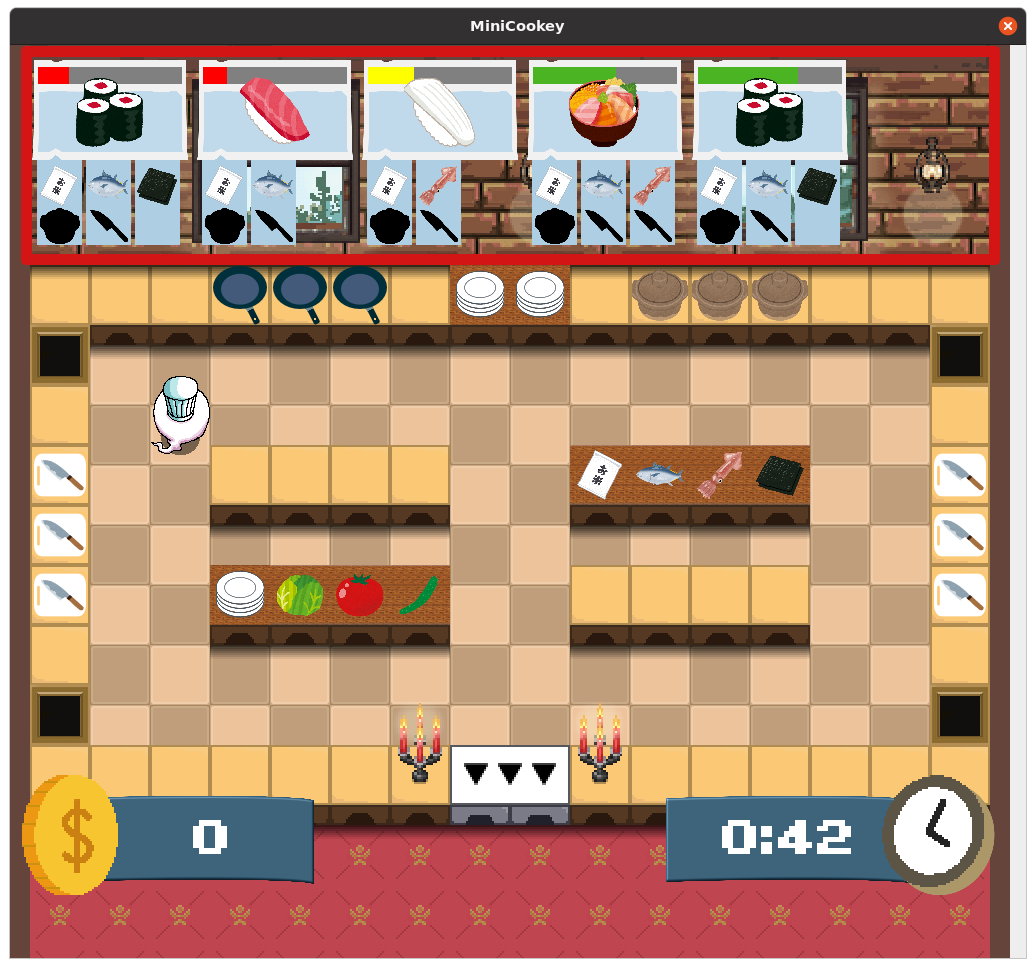
\includegraphics[width=0.4\textwidth,keepaspectratio]{img/d2.png}
    }
  \end{center}
\end{figure}
\begin{figure}[H]
  \begin{center}
    \subfigure[ゲーム画面:加工前]{
      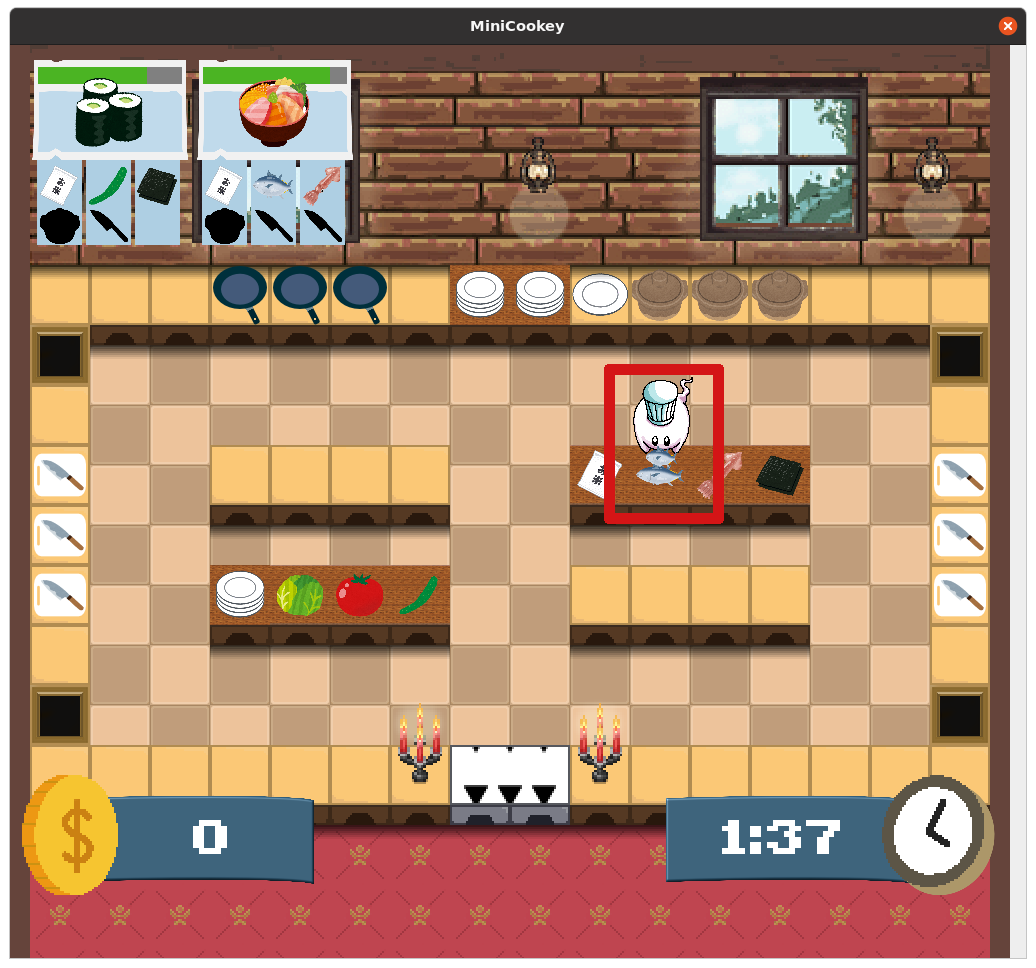
\includegraphics[width=0.4\textwidth,keepaspectratio]{img/e2.png}
    }
    \subfigure[ゲーム画面:加工後]{
      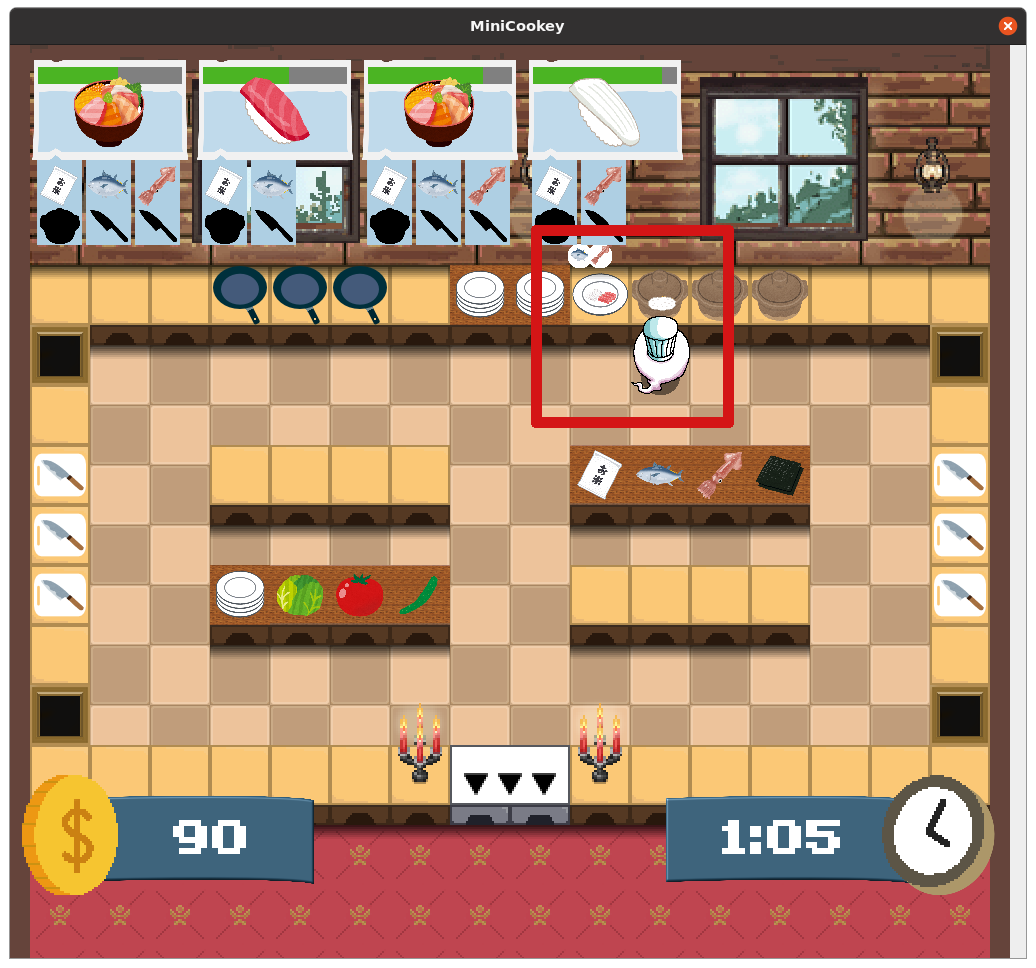
\includegraphics[width=0.4\textwidth,keepaspectratio]{img/f2.png}
    }
  \end{center}
\end{figure}
\begin{figure}[H]
  \begin{center}
    \subfigure[ゲーム画面:組み合わせ後]{
      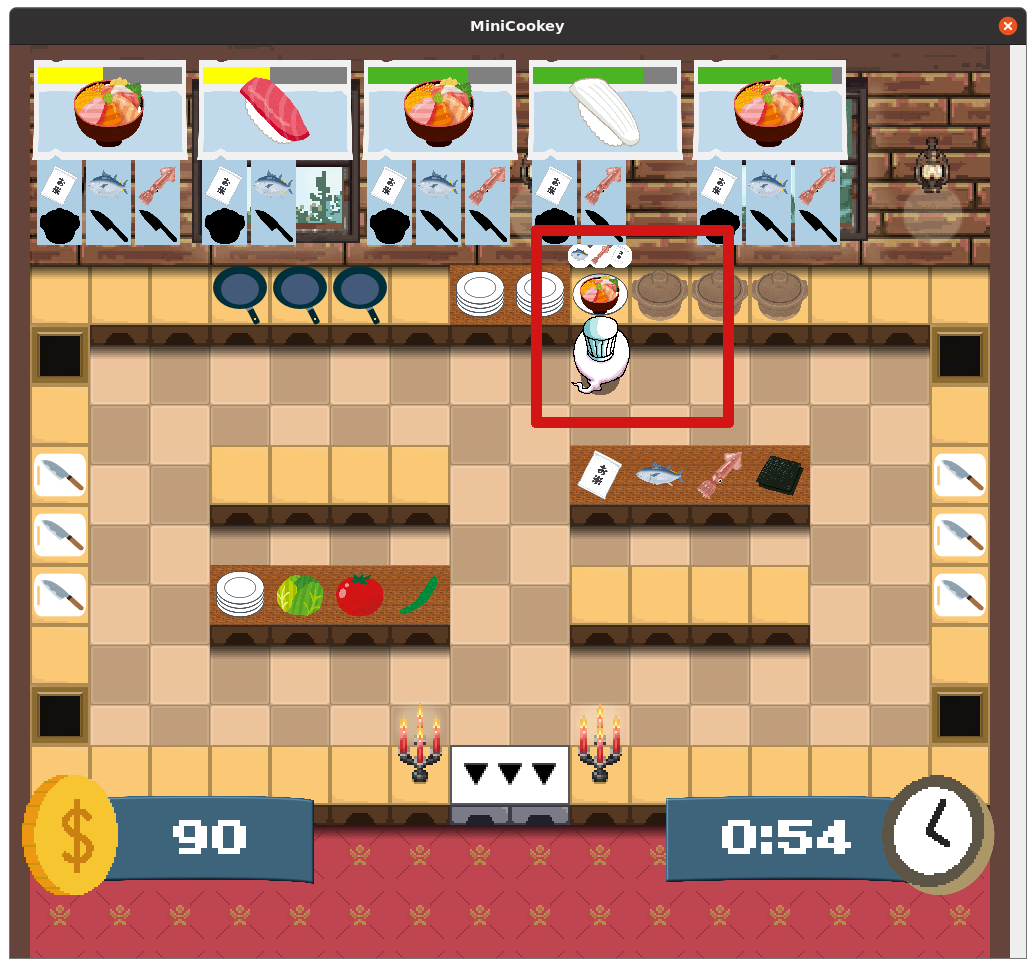
\includegraphics[width=0.4\textwidth,keepaspectratio]{img/g2.png}
    }
    \subfigure[ゲーム画面:提供]{
      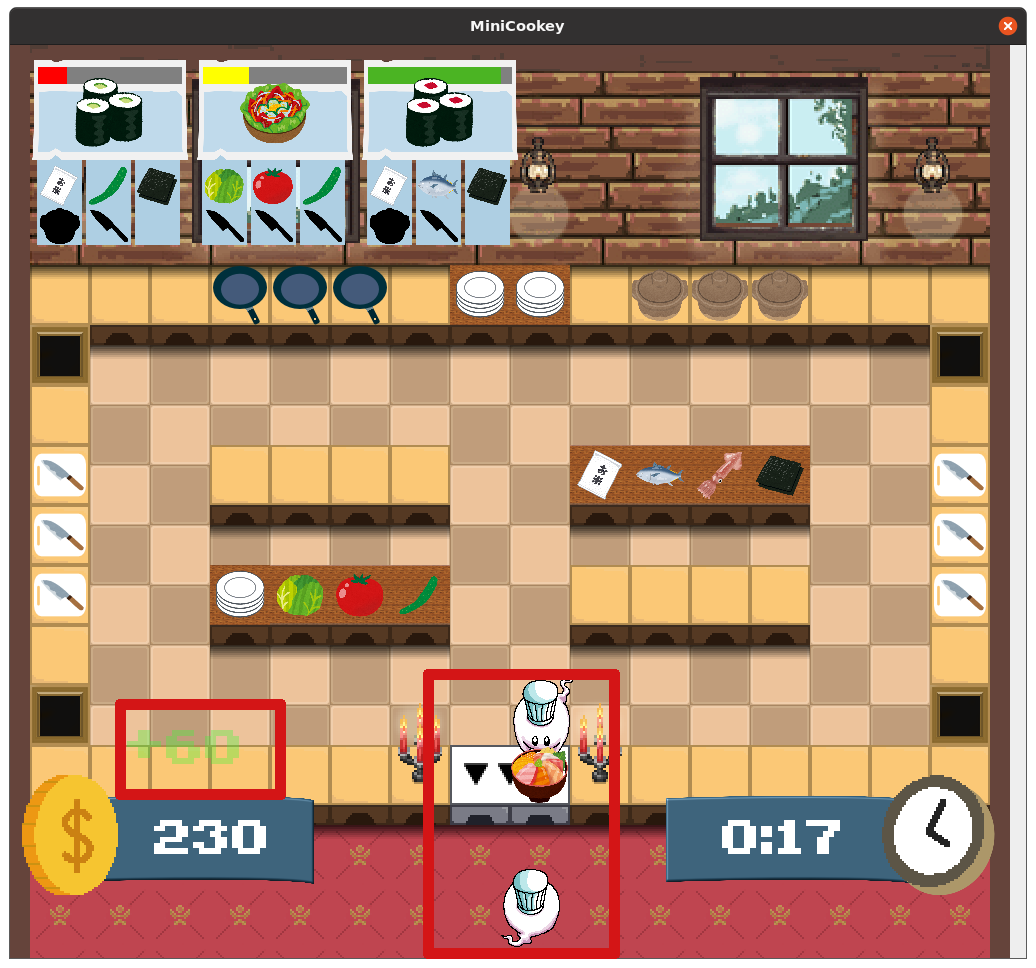
\includegraphics[width=0.4\textwidth,keepaspectratio]{img/h2.png}
    }
  \end{center}
\end{figure}
文責:鈴木

\newpage

\section{考察}
 予定していた以上のものが完成した。%%%%%%%%%%%%%%%%%%%%%%%
文責:吉田

\section{感想}
\subsection*{(米谷祐希)}
%%%%%%%%%%%%%%%%%%%%%%%%%%%
\subsection*{(鈴木早紀)}
 授業前半の個人の課題を最低限しか取り組まなかったために、2人よりJavaを理解していなくて2人に大変な部分を多く任せてしまいました。
2人が進んでやってくれたので感謝しています。画像・音楽の準備やメニューの追加、スライドやレポートは積極的に行えたと思います。
Viewとしての課題は、変数や画像読み込みが多すぎることで、今後食材やメニューの追加を行うときにもひたすらこれを書いていくのは厳しいと感じました。
せめて別ファイルにするなどして、View.java内はシンプルにする方が分かりやすいのかなと思いました。
また、メニューによって食材や調理方法を指定するときは、分量が少なくなるようにif文の順序に工夫はしましたが、
他の班の発表を聞き、csvファイルの読み込みにすることで管理もしやすくなるのかなと考えました。
今回初めて本格的にグループプログラミングを行ったので、共同作業をする大変さや、作業を分割する便利さを知ることができました。
先輩や2人のプログラムを特に参考にして理解を進めることができました。
Javaはこの授業で初めて触ったけれど、半年間という期間を考慮すると大きな成果が得られたなと感じます。
\subsection*{(吉田陽音)}
 授業前半ではJavaの基礎知識やオブジェクト指向について学ぶことができたが、与えられた課題をこなすだけで受け身の学びであった。一方後半の、このゲーム製作では積極的にJavaについての理解を深めていくことができた。
Javaはこの授業で初めて触ったので、ゲーム製作の課題を聞いた当初はそれなりの形にできれば良いかなと思っていたが、実際に製作を進めていくうちに夢中になり、楽しみながらゲームを作ることができた。

 反省点としては、行き当たりばったりな開発となってしまい、クラスが煩雑になってしまったり、メソッドが冗長になってしまったりしたことである。もっと計画的な開発が行えていたら、他の要素を実装する時間が生まれ、より良いゲームを作れたと反省している。

 世の中に存在しているゲームに比べると簡易的なゲームであるが、素人なりにかなりの労力や知識を詰め込んだ気でいたため、友人や家族にこのゲームを見せた時にあまり良いリアクションを得られなかったことがかなりショックであった。この授業では、Javaについてだけでなく、こうした体験を通して学ぶことも多く、さらにはグループ開発を経験できたこともあり、自分にとってかなり有意義であったと実感している。


\newpage
\section*{付録1:操作マニュアル}
\subsection*{(ストーリー)}
 キミはおばけの国のレストランのキッチンで働いているぞ!制限時間内にオーダー通りの料理をたくさん作ろう!目指せ高得点!!
\subsection*{(実行方法)}
 「Java MiniCook」でゲームが開始する。
\subsection*{(操作方法)}
 このゲームはキーボードでキャラクターを操作する。図2にキー操作を示す。W,S,A,Dで上下左右を操作し、Jで取る、Kで置く、スペースキーでアクションを行う。
\begin{figure}[H]
  \begin{center}
  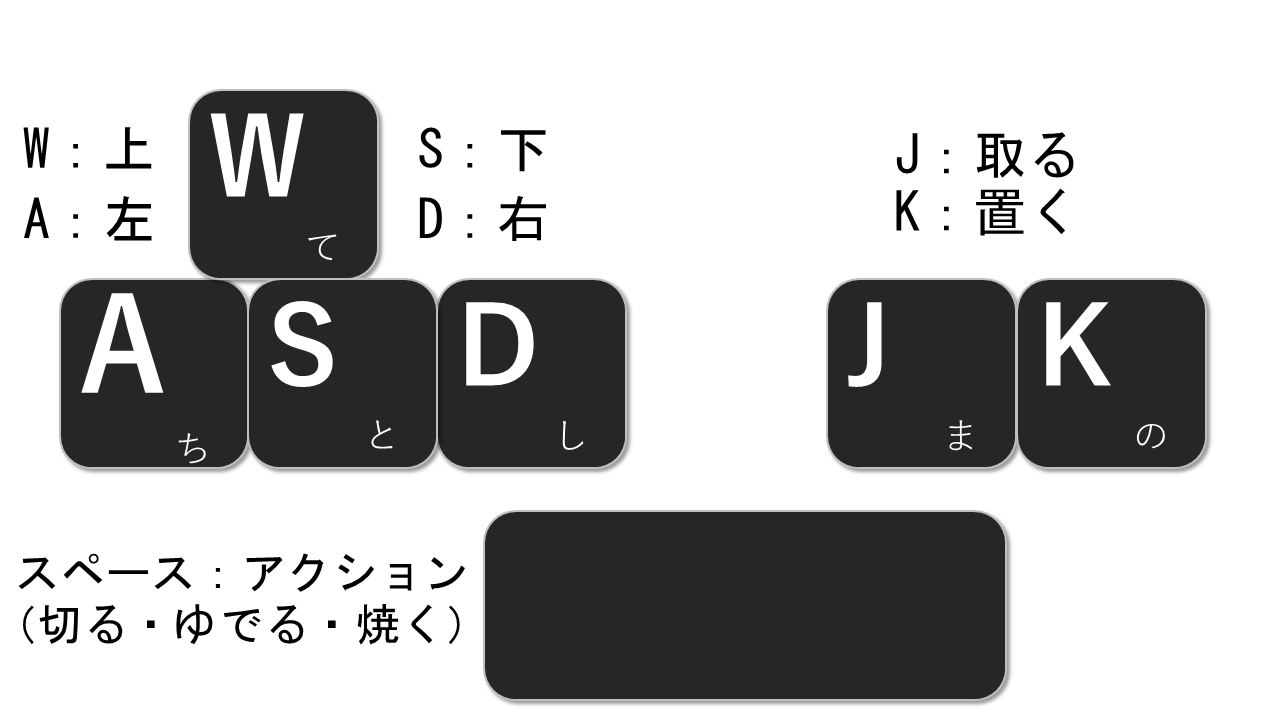
\includegraphics[scale=0.2]{img/key.png}
  \caption{キーボード操作方法}
  \end{center}
\end{figure}
\subsection*{(遊び方)}
\begin{enumerate}
  \item スタート\par
   スタートボタンを押すとゲームが開始する。 
  \item オーダーの確認\par
   まず、画面上部にランダムにオーダーが提示される。オーダーには、使う食材と調理方法が記載されている。各オーダーにはそれぞれ制限時間が設定されており、残り時間はオーダー上のゲージにリアルタイムに表示される。
  \item 食材の調理\par
   次に、オーダーに記載されている食材を、各食材ボックスから取り出す。各食材を持ったまま、各調理器具の前でアクションボタンを押すことで、食材が加工される。
  \item 料理の完成と提供\par
   料理は、加工された食材とお皿を組み合わせることで完成する。それらを組み合わせて料理ができあがれば、提供口に置くことで提供となり、オーダーと一致しているか判定される。一致していれば加点、間違っていれば減点となる。   
  \item リザルト\par
   制限時間がなくなるとリザルト画面に遷移する。スコアとランクが表示される。リザルトを押せばもう一度ゲームが開始する。
\end{enumerate}
\subsection*{(ゲーム画面)}
 ゲーム画面は図3のように、オーダー、キャラクター、食材・皿ボックス、スコア、調理器具、提供口、制限時間で構成されている。
\begin{figure}[H]
  \begin{center}
  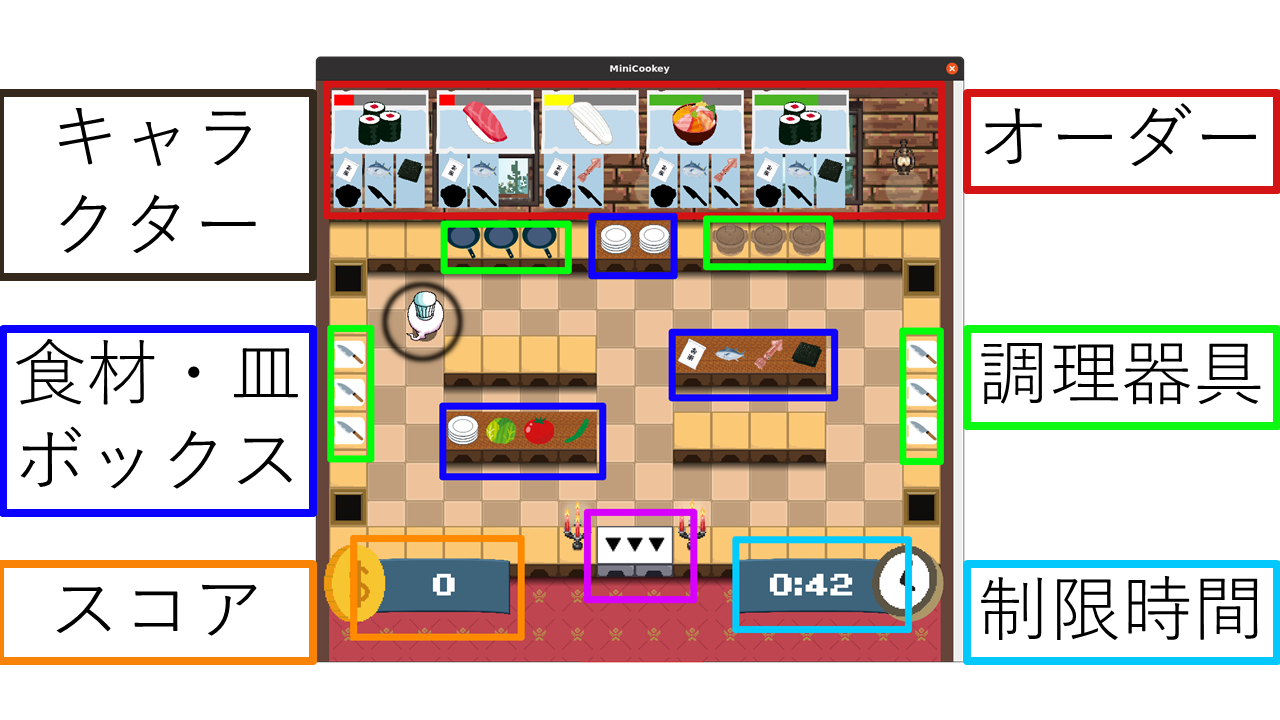
\includegraphics[scale=0.3]{img/game.png}
  \caption{ゲーム画面の説明}
  \end{center}
\end{figure}
\subsection*{(データ)}
\begin{itemize}
  \item メニュー一覧\par
    \begin{itemize}
      \item マグロ握り
      \item イカ握り
      \item 海鮮丼
      \item カッパ巻
      \item 鉄火巻き
      \item サラダ
    \end{itemize}
  \item 調理器具一覧\par
    \begin{itemize}
      \item 包丁
      \item 鍋
    \end{itemize}
  \item 食材一覧\par
    \begin{itemize}
      \item マグロ
      \item イカ
      \item 米
      \item 海苔
      \item キャベツ
      \item トマト
      \item キュウリ
    \end{itemize}     
\end{itemize}
文責:鈴木



\newpage
\section*{付録2:プログラムリスト}
以下にプログラムリスト全体を記述する。
\lstset{
    language=Java,
    inputencoding=utf8,
    %basicstyle=\ttfamily\scriptsize,
    basicstyle=\ttfamily\tiny,%最小文字、見にくいかも
    extendedchars=false,%日本語のためらしい
    breaklines=true,%長い行折る
    numbers=left,%行番号を左側に
    numberstyle=\tiny,%行番号サイズ
    stepnumber=1, %1行ごとに番号を表示
    frame=single, %枠
    tabsize=4 %タブの幅
}
\begin{itemize}
  \item MiniCook
  \lstinputlisting{../MiniCook.java}
  \item Model
  \lstinputlisting{../Model.java} 
  \item View
  \lstinputlisting{../View.java} 
  \item Controller
  \lstinputlisting{../Controller.java}  
  \item Order
  \lstinputlisting{../Order.java}
  \item Player
  \lstinputlisting{../Player.java}
  \item Start
  \lstinputlisting{../Start.java}
  \item Result
  \lstinputlisting{../Result.java}
  \item Meal
  \lstinputlisting{../Meal.java}
  \item Other
  \lstinputlisting{../Other.java}
  \item AudioManager
  \lstinputlisting{../AudioManager.java} 
\end{itemize}
\normalsize
文責:米谷・鈴木・吉田

\end{document}

\begin{comment}
\end{comment}